\chapter{Dominio del progetto}

\section{Introduzione}
Motology è un ontologia riguardante il mondo delle competizioni motociclistiche, improntata particolarmente sul Motomondiale. Nasce con lo scopo di aiutare appassionati, meccanici, piloti, cronisti etc. ad ottenere informazioni e statistiche composite riguardanti il loro sport preferito. L'ontologia nasce a scopo consultativo, tuttavia potenzialmente potrebbe essere impiegata per derivare nuovi dati o studiare correlazioni ed allenare modelli di intelligenza artificiale a prevedere trend futuri. 
\\\\
La prima fase della modellazione ha coinvolto la definizione di tutte le entità che compongono l'ontologia, partendo dalle classi, proprietà e vincoli. In una seconda fase dopo aver verificato che il sistema inferisse nuove informazioni da ciò che era stato definito, sono state formulate diverse query in modo da mostrare le potenzialità dell'ontologia e da ottenere informazioni derivate in modo semplice, senza dover svolgere numerose ricerche online dovendosi trovare ad unificare dati sparsi ed eterogenei. L'immagine seguente riassume brevemente l'ordine di grandezza di Motology:
\\
\begin{figure}[H]
    \begin{center}
        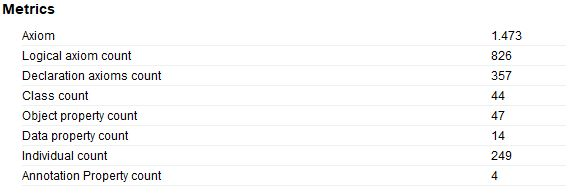
\includegraphics[scale=0.9]{img/statistiche.jpg}
       \caption{Un pò di numeri riguardanti Motology} 
    \end{center}
\end{figure}

In seguito illustreremo le classi principali, citeremo le ontologie esterne impiegate per modellare determinati concetti di natura più generale rispetto al dominio in oggetto ed infine faremo una panoramica delle tecnologie adottate per lo sviluppo di Motology.

\newpage

\section{Design: scelta delle Classi}
Nella prima parte della definizione dell'ontologia è stato fondamentale delineare il "perimetro" ed il livello di dettaglio di cui dotare Motology allo scopo di non trattare determinati temi in maniera troppo approfondita per mantenere solamente dati utili a formare interrogazioni interessanti. Le classi che ci hanno aiutato a definire questi aspetti sono state:

\subsection{moto:GranPremio}
Classe che rappresenta (da wikipedia) "un insieme di gare di velocità su pista delle due ruote motorizzate che si svolge su un apposito circuito", nonchè il soggetto principale di Motology. La peculiarità di un gran premio motociclistico è che si svolge in un singolo circuito per ogni nazione (es. Mugello per il gran premio d'Italia), comprende tutte le competizioni, gare, qualifiche e prove libere, per ogni campionato (es. Moto2, MotoGP). Nel successivo capitolo spiegheremo più in dettaglio come sono stati modellati tutti questi concetti, partendo da quello di Gran Premio. Di seguito possiamo vedere come risulta la struttura finale dell'ontologia:
\\\\
\begin{figure}[H]
    \begin{center}
        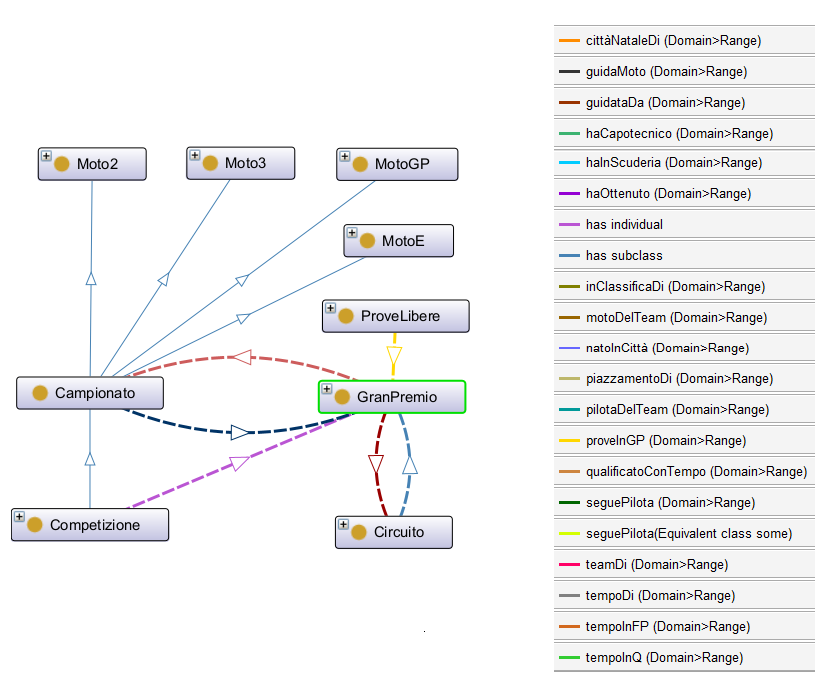
\includegraphics[scale=0.9]{img/gran premio.png}
       \caption{Ontograph riguardante il Gran Premio} 
    \end{center}
\end{figure}

\newpage

\subsection{moto:Pilota}
 La scelta di creare una classe separata per i piloti è stata motivata dalla necessità di modellare una componente fondamentale di un evento motociclistico, la presenza di un protagonista, delineato appunto da Pilota. Questa classe, oltre a consentire di specificare attributi e relazioni uniche per questo ruolo specifico, ci ha permesso di riflettere sugli altri ruoli della "Persona" all'interno di questo ambito. Abbiamo quindi deciso di modellare il concetto di Persona, andando a riutilizzare la definizione presente in FOAF per modellare anche altre figure, come quelle di Capo tecnico, Team Manager, ed alcuni casi particolari di pilota detti "Leggende" (coloro che hanno vinto almeno un gran premio per ogni campionato). Queste figure saranno spiegate in maggior dettaglio nel capitolo successivo.
\\\\
\begin{figure}[H]
    \begin{center}
        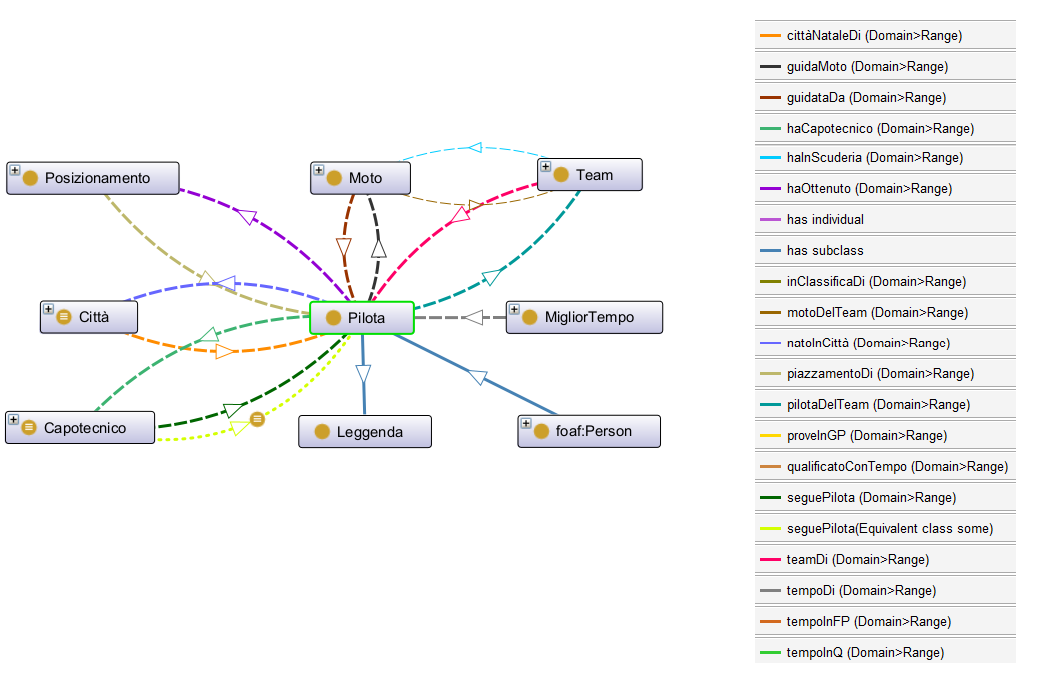
\includegraphics[scale=0.75]{img/pilota.png}
       \caption{Ontograph riguardante il Pilota} 
    \end{center}
\end{figure}

\newpage

\subsection{moto:Moto}
Ulteriore aspetto che abbiamo ritenuto fondamentale per ottenere statistiche e recommendation esaustive (oltre all'evento "Gran Premio" e la persona "Pilota") è quello del veicolo impiegato in questo tipo di competizioni, la Moto. Le moto da gran premio sono prototipi da competizione, sviluppate specificamente per le corse e non sono disponibili sul mercato. Questa classe ci permette di scendere nei dettagli più tecnici ed eventualmente di rendere estendibile Motology da chiunque volesse modellare scelte dello staff ingegneristico (ad esempio la scelta delle gomme basata sulle condizioni climatiche e meteorologiche). Analizzando questa classe e le sue proprietà in fase di progettazione abbiamo deciso di modellare altri concetti strettamente collegati a quello di moto, come il tipo di motore ed alcune sue caratteristiche e l'azienda produttrice del prototipo, che coincide spesso con la scuderia della moto.
    
\begin{figure}[H]
    \begin{center}
        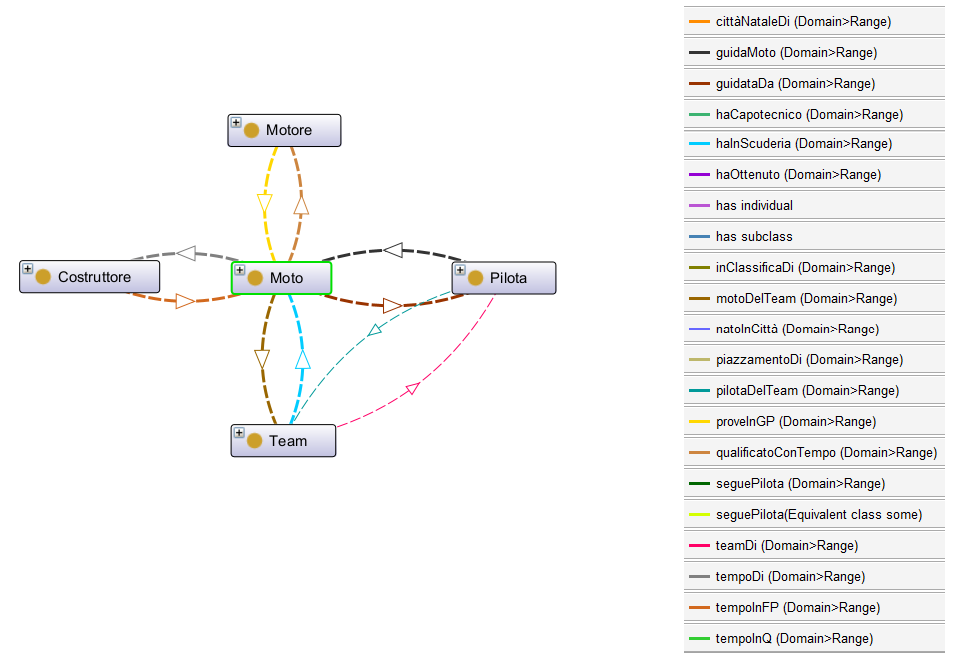
\includegraphics[scale=0.8]{img/moto.png}
       \caption{Ontograph riguardante la Moto} 
    \end{center}
\end{figure}

\newpage

\section{Impiego di ontologie esistenti}
Le Ontologie impiegate all'intero di questo progetto per modellare concetti già noti e ampiamente trattati sono:

\begin{itemize}
    \item \textbf{foaf:person} il motivo principale di questa scelta è stato quello di sfruttare la ricchezza concettuale offerta da FOAF (acronimo di Friend Of A Friend) per rappresentare le informazioni relative agli individui coinvolti nel contesto di Motology, tra cui troviamo i piloti, i capi tecnici ed i team manager. Questa scelta di integrazione tra Motology e FOAF ci consente di beneficiare dell'interoperabilità con altre ontologie e applicazioni semantiche che fanno uso di FOAF come standard per la rappresentazione delle informazioni personali e sociali.

    \item \textbf{dbo:nation e dbo:city} L'integrazione delle ontologie dbo:nation e dbo:city in Motology è stata effettuata per consentirci di modellare in modo completo e accurato informazioni di natura geografica coinvolte nel nostro sistema. Questa scelta è motivata dalla necessità di rappresentare proprietà come la nazionalità dei piloti, dei costruttori, il luogo in cui è presente un circuito e le località delle gare.
\end{itemize}

\section{Tecnologie e linguaggi adottati}
I vincoli implementativi hanno influenzato l'intero processo di realizzazione del sistema, determinando l'adozione di determinati linguaggi di programmazione e/o strumenti software specifici. Nel contesto dello sviluppo di questo progetto, ci siamo uniformati ad i seguenti vincoli tecnologici:

\begin{itemize}
    \item \textbf{RDF, RDF Schema e OWL:} Queste tecnologie sono state utilizzate per modellare il dominio del sistema. L'adozione di RDF (Resource Description Framework), RDF Schema e OWL (Web Ontology Language) ci ha permesso di rappresentare in modo strutturato e semantico le informazioni del dominio.
    \item \textbf{SPARQL:} Abbiamo adottato SPARQL come linguaggio di interrogazione all'ontologia. SPARQL ci consente di formulare query ottenendo risultati pertinenti in base alle nostre esigenze.
    \item \textbf{SWRL:} abbiamo impiegato SWRL (Semantic Web Rule Language) per esprimere regole di logica aggiuntive, come regole di inferenza che hanno permesso di dedurre nuove informazioni a partire dai dati esistenti nell'ontologia. Questo ha reso possibile l'applicazione di ragionamenti automatizzati e l'estensione delle capacità di inferenza del nostro sistema.
\end{itemize}